% THIS IS AN EXAMPLE DOCUMENT FOR VLDB 2012
% based on ACM SIGPROC-SP.TEX VERSION 2.7
% Modified by  Gerald Weber <gerald@cs.auckland.ac.nz>
% Removed the requirement to include *bbl file in here. (AhmetSacan, Sep2012)
% Fixed the equation on page 3 to prevent line overflow. (AhmetSacan, Sep2012)

\documentclass{vldb}
\usepackage{graphicx}
\usepackage{balance}  % for  \balance command ON LAST PAGE  (only there!)
%\usepackage{notoccite}


\begin{document}

% ****************** TITLE ****************************************

\title{A Review of Deep Convolutional Neural Networks in Robotic Grasps Detection}

% possible, but not really needed or used for PVLDB:
%\subtitle{[Extended Abstract]
%\titlenote{A full version of this paper is available as\textit{Author's Guide to Preparing ACM SIG Proceedings Using \LaTeX$2_\epsilon$\ and BibTeX} at \texttt{www.acm.org/eaddress.htm}}}

% ****************** AUTHORS **************************************

% You need the command \numberofauthors to handle the 'placement
% and alignment' of the authors beneath the title.
%
% For aesthetic reasons, we recommend 'three authors at a time'
% i.e. three 'name/affiliation blocks' be placed beneath the title.
%
% NOTE: You are NOT restricted in how many 'rows' of
% "name/affiliations" may appear. We just ask that you restrict
% the number of 'columns' to three.
%
% Because of the available 'opening page real-estate'
% we ask you to refrain from putting more than six authors
% (two rows with three columns) beneath the article title.
% More than six makes the first-page appear very cluttered indeed.
%
% Use the \alignauthor commands to handle the names
% and affiliations for an 'aesthetic maximum' of six authors.
% Add names, affiliations, addresses for
% the seventh etc. author(s) as the argument for the
% \additionalauthors command.
% These 'additional authors' will be output/set for you
% without further effort on your part as the last section in
% the body of your article BEFORE References or any Appendices.

\numberofauthors{3} %  in this sample file, there are a *total*
% of EIGHT authors. SIX appear on the 'first-page' (for formatting
% reasons) and the remaining two appear in the \additionalauthors section.

\author{
% You can go ahead and credit any number of authors here,
% e.g. one 'row of three' or two rows (consisting of one row of three
% and a second row of one, two or three).
%
% The command \alignauthor (no curly braces needed) should
% precede each author name, affiliation/snail-mail address and
% e-mail address. Additionally, tag each line of
% affiliation/address with \affaddr, and tag the
% e-mail address with \email.
%
% 1st. author
\alignauthor
Shehan Caldera\\
       \affaddr{School of Engineering}\\
       \affaddr{Edith Cowan University}\\
       \affaddr{Australia}\\
       \email{shelessa@our.ecu.edu.au}
% 2nd. author
\alignauthor
A/Prof. Alex Rassau\\
       \affaddr{School of Engineering}\\
       \affaddr{Edith Cowan University}\\
       \affaddr{Australia}\\
       \email{a.rassau@ecu.edu.au}
% 3rd. author
\alignauthor
Dr Douglas Chai\\
       \affaddr{School of Engineering}\\
       \affaddr{Edith Cowan University}\\
       \affaddr{Australia}\\
       \email{d.chai@ecu.edu.au}
}
% There's nothing stopping you putting the seventh, eighth, etc.
% author on the opening page (as the 'third row') but we ask,
% for aesthetic reasons that you place these 'additional authors'
% in the \additional authors block, viz.

% Just remember to make sure that the TOTAL number of authors
% is the number that will appear on the first page PLUS the
% number that will appear in the \additionalauthors section.


\maketitle

\begin{abstract}
The scientific community has recently experienced numerous developments in the area of intelligent machines because of the rapid improvement in data-based learning algorithms. Presently, Deep Learning (DL) is identified as capable of classification, recognition, and localisation applications of computer vision. Many recent studies have focused on implementing learning algorithms in robotic applications in Unstructured Environments (UE). Due to the variable nature of a UE, analytical robotic solutions can be expensive. Deep Convolutional Neural Network (DCNN) is the generic term for most of these learning algorithms. This paper reviews DCNN algorithms that appear in most recent robotic grasping work.
\end{abstract}

\section{Introduction}
Humans perform better than robots in learning to grasp objects. 

\section{Grasp Representation}
General purpose robots in a human-robot collaborative work environment need to have the ability to manipulate objects in the physical world. Object grasping is challenging in its own factors such as different object shapes and unlimited object poses. Successful grasp detection system should be able to overcome this challenge to predict valuable results. Unlike robots, humans almost immediately know how to grasp a given novel object. Robotic grasping performs well below the human object grasping benchmarks but continuous effort is made to improve considering the higher demand. Robotic grasping has 3 stages \cite{sulabh}.
\begin{enumerate}
    \item Grasp detection
    \item Grasp planning
    \item Hardware Control
\end{enumerate}
Grasp detection recognises the grasping point(s) of a given image including the pose of the grasp in the image \cite{mahler}. The pose describes the grasp orientation on the image plane. Grasp planning discusses the path planning that is required to achieve a successful grasp including obstacle avoidance if necessary. Hardware control implies the necessary programming or interfacing required to achieve the robotic manipulation for object grasping. As we humans use vision in such tasks as object grasping, robots use visual sensors or perception in the same task. Therefore grasp detection can be defined as given a dataset from a perception sensor, finding of the grasping points using ground truth data as a guideline if available. Different literature define robotic grasps for objects in various manners. Some of the promising approaches will be reviewed here.
\\ \\
Using a supervised learning approach, Saxena et al. \cite{saxena_2006} investigated a regression learning method to infer the 3-d location of the grasping point in a Cartesian coordinate system. Considering the camera position uncertainty into account Saxena et al. \cite{saxena_2006} also used a probabilistic model over possible grasping points. To further in their investigation, they had descritised the the 3-d workspace in order to find the grasping point $g$, given by
\begin{equation}
    g = (x,y,z)
\end{equation}
To infer the 3 coordinates, they used two or more images of the same object \cite{saxena_2006}. As shown in Figure \ref{fig:saxena-regions}, furthering their investigation, Saxena et al. \cite{saxena-2008} defined graspable regions of objects as grasping points for their learning algorithm to infer a 3-d grasping point.
\begin{figure}[!h]
    \centering
    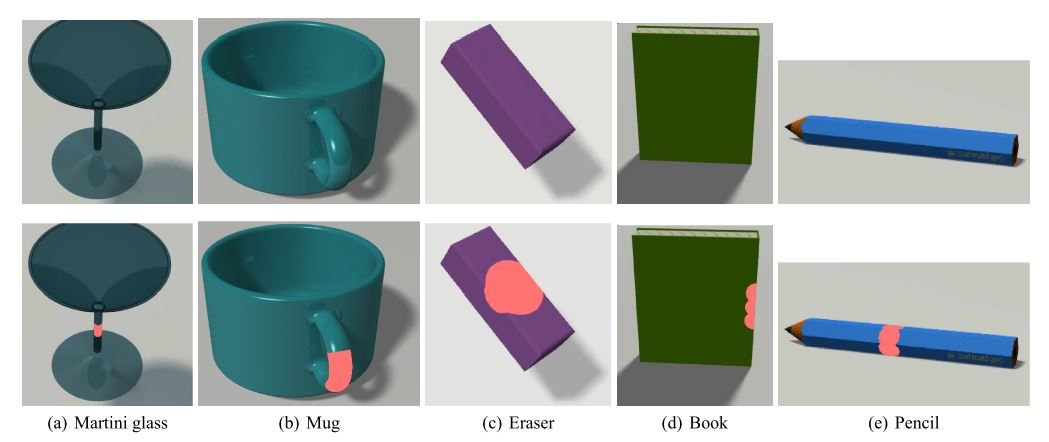
\includegraphics[width=0.5\textwidth]{Saxena_2008_graspingRegions}
    \caption{Five object classes used for training with their grasping points marked on the images. Objects are a Martini glass, Mug, Eraser, Book, and a Pencil \protect\cite{saxena-2008}.}
    \label{fig:saxena-regions}
\end{figure}
Most of these approaches were investigated with RGB colour images and RGB simulated images before the introduction of the depth sensors which has improved all detection work including the grasp detection since then.
\\ \\
Considering the challenge of grasping novel objects, one first has to define the problem space accurately to tackle the problem in a proper manner. Point defined grasps only suggest where to grasp it. It does not determine how wide the gripper ends have to be opened nor the orientation of the gripper ends. Taking this into account Jiang et al. \cite{jiang} has proposed a method to detect robotic grasp configurations in 3D space using RGB-D images. According to Jiang et al. \cite{jiang} a grasping configuration has a seven dimensional representation. The grasp representation from Jiang et al. \cite{jiang} contains \textbf{Grasping point}, \textbf{Grasping orientation}, and \textbf{Gripper opening width}. In 3D space the actual grasp representation, $G$ can be stated as in Equation \ref{eqn:jiang_etal}.
\begin{equation}
\label{eqn:jiang_etal}
G = (x, y, z, \alpha, \beta, \gamma, l)
\end{equation}
Jiang et al. \cite{jiang} represented a grasp as an oriented rectangle in the image plane. The rectangle edges shown in Figure \ref{fig:jiang-rectangle} in blue colour represented the jaws of the gripper. The red coloured edges represented the opening or closing width of the gripper along with the direction of the motion. 
\begin{figure}[!h]
	\centering
	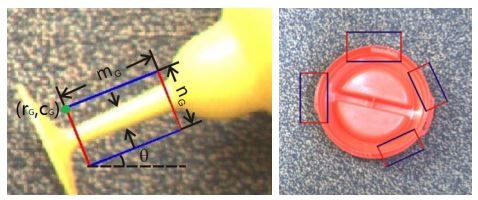
\includegraphics[width=0.5\textwidth]{grasping-rectangle-jiang}
	\caption{Grasping rectangle representation. The upper-left corner $(r_G,c_G)$, length $m_G$, width $n_G$ and its angle from the x-axis, $\theta_G$. For some objects, like a red coloured lid in the right image, there can be multiple possible grasping rectangles \protect\cite{jiang}.}
	\label{fig:jiang-rectangle}
\end{figure}
Simplifying the seven dimensional grasp rectangle representation by Jiang et al. \cite{jiang}, Lenz et al. \cite{lenz} proposed a five dimensional representation similar to the approach by Jiang et al. \cite{jiang}. This was based on the assumption of a good 2D grasp being able to be projected back to 3D space. While Lenz et al. \cite{lenz} failed to evaluate their approach, Redmon et al. \cite{redmon} confirmed the validity of the method with their own results. Redmon et al. \cite{redmon} reassured the statements by Jiang et al. \cite{jiang} and Lenz et al. \cite{lenz}, that detection of grasping points in this manner was analogous to object detection methods in computer vision but with an added term for the gripper orientation.
\\ \\
Adapting the method of \cite{jiang,lenz}, Redmon et al. \cite{redmon} presented a slightly updated representation of a grasp rectangle as shown in Figure \ref{fig:redmon-rectangle}.
\begin{figure}[!h]
	\centering
	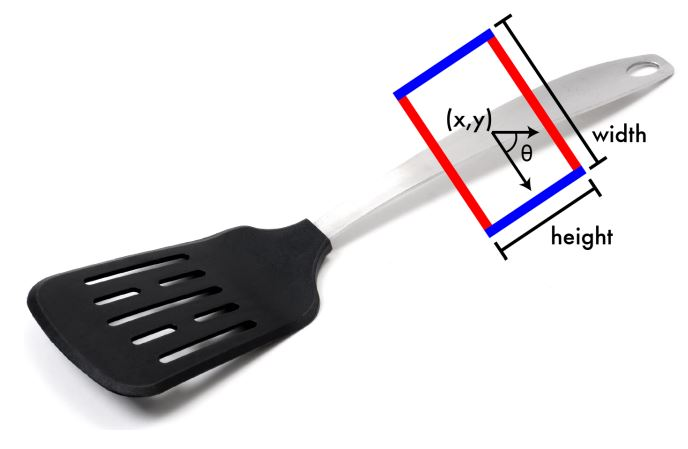
\includegraphics[width=0.4\textwidth]{redmon-rectangle}
	\caption{Grasp rectangle by Redmon et al. \protect\cite{redmon}. Where $(x, y)$ is the center of the rectangle, $\theta$ is the orientation of the rectangle relative to the horizontal axis, $h$ is the height, and $w$ is the width \protect\cite{redmon}.}
	\label{fig:redmon-rectangle}
\end{figure}
This modified rectangle grasp representation has been used few late publications proving its usefulness. In their work to use deep learning algorithms for robotic grasping detection, Sulabh et al. \cite{sulabh} have used the grasp rectangle proposed by Redmon et al. \cite{redmon}. A very recent online project page \cite{redmon} has cited the Redmon grasp rectangle in their work.
\\ \\
Inspired by the methods of Reinforcement Learning \cite{mnih} Pinto et al. \cite{pinto} presented a self-supervising algorithm for collecting data for learning to detect robotic grasps. Pinto et al. \cite{pinto} stated that manually labelled data would not be scalable for various applications therefore application specific data is need for the individual application. Considering the amount of data that might require for such a method, Pinto et al. \cite{pinto} presented a minimised representation of the grasp neglecting the gripper opening width. Given the grasping point $G=(x,y)$, Pinto et al. \cite{pinto} prposed a method to predict the grasp orientation $\theta$. According to Pinto et al. \cite{pinto} a grasp, $G$ can defined as $G = (x, y, \theta)$.   
\section{Grasp Detection}
\section{Neural Network Architectures}
\section{Robotic Grasping Databases}
\section{Grasp Planning and Simulation}
Also include results of the published work
\section{Conclusion}

\bibliographystyle{ieeetr}
\bibliography{vldb_sample}

%\begin{appendix}
%Necessary appendices will be added at the end.
%\section{Results of DL with Recent Works}
%\end{appendix}


\end{document}

